


\documentclass[12pt]{article}
%\usepackage[a4paper]{geometry}
%\usepackage[myheadings]{fullpage}
%\usepackage{fancyhdr}
%\usepackage{lastpage}
%\usepackage{graphicx, wrapfig, subcaption, setspace, booktabs}
%\usepackage[T1]{fontenc}
%\usepackage[font=small, labelfont=bf]{caption}
%\usepackage{fourier}
%\usepackage[protrusion=true, expansion=true]{microtype}
\usepackage[english]{babel}
\usepackage[utf8]{inputenc}
\usepackage{graphicx}
%\usepackage{sectsty}
%\usepackage{url, lipsum}



%-------------------------------------------------------------------------------
% HEADER & FOOTER
%-------------------------------------------------------------------------------

%-------------------------------------------------------------------------------

\title{Jordskælv simulation - DatF eksamen 2018}

\date{4. Februar 2018}

\author{
		Navn: Morten Dalfoss \\
		KU-ID: krs476 \\ }


\begin{document}
\graphicspath{ {F:/Uni/DatF/datfeksamen/Morten} }

\maketitle
\tableofcontents
\newpage

\section{Introduktion}
I Denne rapport redegøres for et program, skrevet i Matlab, der forsøger, at simulere et jordskælv via en meget simpel model, der bygger på en SOC model, samt numeriske løsninger til denne. Derudover illustreres brugen af dette program.
I modellen antages det at et jordskælv forsages af to plader, der er i forbindelse med hindanden via nogle klodser, der hver især er forbundet til naboklodser, samt den øverste plade, med fjedre. Når den øverste plade forskubbes, iforhold til en eller flere af klodserne, vil den resulterende kraftpåvirkning fra fjedren der er fastgjort til den øverste plade, få klodserne til at bevæge sig, hvis klodsens friktionskraft bliver overskredet. Dette vil så få naboklodserne til at blive udsat for større kraft, og igen, hvis friktionskraften bliver overskredet, give anledning til en kædereaktion af forskubbelser, indtil en ny stabil konfiguration er opnået. Dette er modellen der repræsenterer jordskælvet. Ud fra afstanden hver klods flytter sig, samt friktionskraften, kan man udregne den frigivne energi, og kan dermed både bestemme størrelsen af skælvet, samt antallet af involverede klodser.

\subsection{Løsningsmodellen}

Løsningsmodellen er en 2-D simulation af ovenstående model. Der bygger på en række antagelser. Det antages, at der er lige langt mellem alle klodser i modellen, altså alle fjedre mellem klodser er lige lange denne karakteristiske længde er betegnet $l_0$. yderligere antages det at friktionskraften for hver blok, er den samme, men med en standardafvigelse på 5\%. Fjedrene der forbinder blokkene, antages også at have samme fjederkonstant for alle fjedre i x retningen, samt alle fejdre i y retningen. Der antages også at der er periodiske grænsebetingelser, hvilket også er afspejlet af koden. Slutteligt antages det, at hver ustabil blok der bliver sat i bevægelse, bevæger sig i rening af den resulterende kraft fra alle fjedre, indtil det punkt hvor størrelsen er lig brøkdelen $\alpha$ af friktionskraften.
\begin{equation}
	|F_{fjedre}| = \alpha * |F_{friktion}|
\end{equation}

 $\alpha$ er sat til 0.75 $\pm$ 5\%. Dette gøres for at opnå et mere stabilt system. Og er også vigtigt for modellen, da det antages at hver klods kun bevæger sig én gang, og derfor ikke skal være på randen til bevægelse igen, når den stopper.

\newpage

\section{Programmet}
 
\subsection{Opbygning}
Programmets grundlæggende logik er skitseret i følgende flow-diagram:

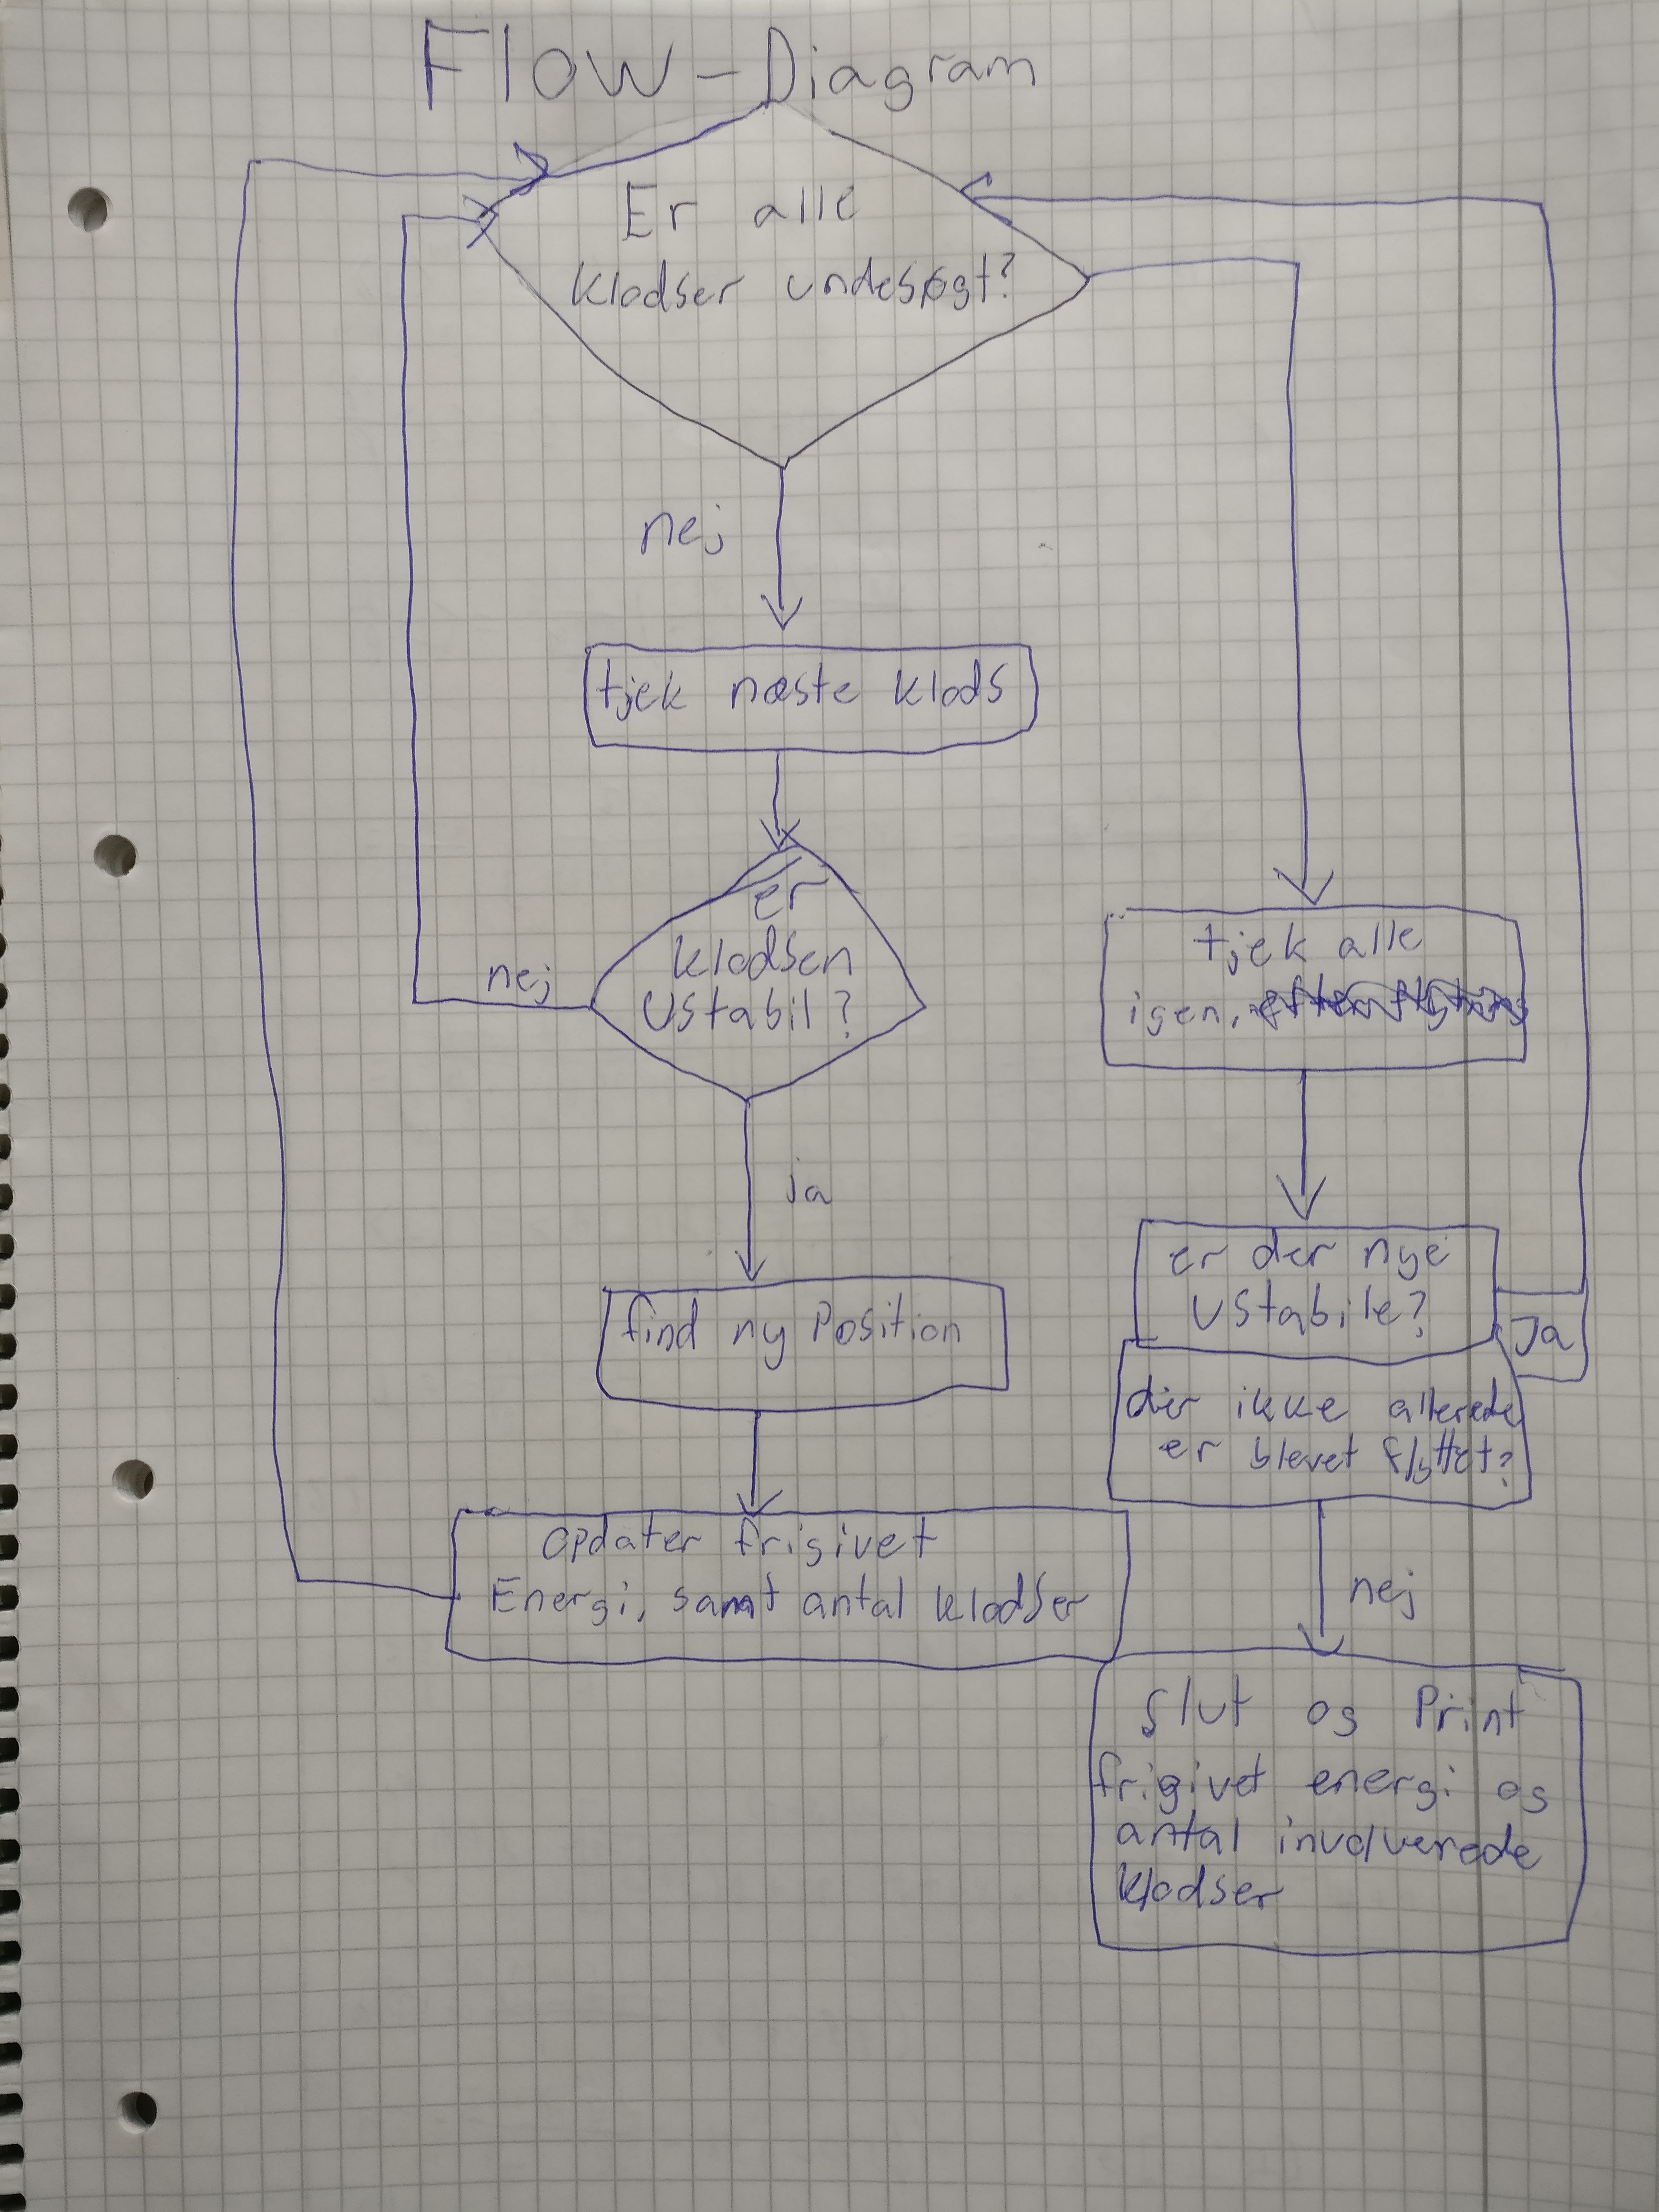
\includegraphics[scale=0.1]{F:/Uni/DatF/datfeksamen/Morten/flowdiagram.jpg}

\newpage

Programmet er struktureret således, at man først tjekker kraften der påvirker alle klodser, og ud fra den kraft, bestemmer om de er ustabile eller ej, hvis de er ustabile, bliver de flyttet til deres nye position. Efter dette er gjort, tjekkes alle klodser igen, for at tjekke for, om den nye position nogle af klodserne har fået, har resulteret i at andre klodser er blevet ustabile. Dette gentages indtil, alle klodser på et tidspunkt er blevet tjekket og der ikke r kommet nogen nye ustabile klodser. Nu er systemet i en stabil tilstand.

En af udfordringerne ved dette program, er at lave en passende flytte funktion. I mit program er det gjort således at forskellen mellem størrelsen af kraftvektoren fra fjedrene og friktionskraften ganget med $\alpha$ og ganget med 0.02, bruges som scale, for hvor meget den givne klods skal flytte sig. Klodsen bliver derefter rykket parallelt med kraftvektoren, og kraften den påvirkes af udregnes på ny. Denne process gentages indtil klodsen er i en postion hvor den er stabil, som defineret i introduktionen.

For at holde styr på hvilke variable der hørte til hvilken klods, besluttede jeg mig for, at benytte mig af objekt orienteret programmering. Dette ville også gøre det muligt at definere fjederkonstanter, fjederlængder m.m individuelt, for hver blok, samt hver enkelt fjeder på den givne blok. Dette overstiger imidlertid målet for denne opgave, men er ikke desto mindre muligt.
For at holde styr på hvilket object der tilhørte hvilken blok, uden at skulle gøre brug af en masse forskellige navne og indekser, strukturerede jeg mine objekter i et objekt array. Dette medførte at jeg kunne tilgå et objekt i postionen (i,j) af min klods matrix via objarray(i,j).value

\subsection{Hvordan bruges det}
Programmet kan køres som det er, men der er et par justerbare variable. Disse findes i sektionerne 'Justerbare variable' samt 'Valg af ryk i øvre plade $ l_{p} $'.
under justerbare varialbe, kan man vælge størreslen af det array af klodser man vil simulere, standard sat til 50x50. Derudover kan man her fjerne udkommenteringen af en linje, der gør at simuleringen startes med at den øverste plade forskubbes en fast afstand for alle klodser involveret. Dette er som sagt udkommenteret med et '\%', da dette ikke er den mest spændende måde at gøre det på, efter min mening. 
Den bedste måde at gøre systemet ustabilt på, findes i sektionen 'Valg af ryk i øvre plade $ l_p $. Her findes 15 (kan justeres i det simple for-loop der er), tilfældige klodser, der hver især får en tilfældig, forskydning af den øverste plade. Dette medfører at man på de to producerede flot, 'foerskaelv' og 'efterskaelv', kan se at der opstør pertubationer i klodsernes position, 15 forskellige steder, og med forskellige størrelser.

Forskydningen af den øverste plade, er tilfældig, inden for et passende interval, da programmets funktionalitet bryder ned, hvis forskydingen bliver for stor. Dette skyldes at kraften bliver for stor, og de små inkrementer klodserne bliver ykket i, simpelthen bliver for store. Dette skal man tage til overvejelse, hvis man manuelt vælger en forskydning.


\subsection{Programmet i brug}

Nedenfor ses postionen af alle klodser, plottet før forskydning af det øverste lag.
\begin{figure}[!h]
\centering
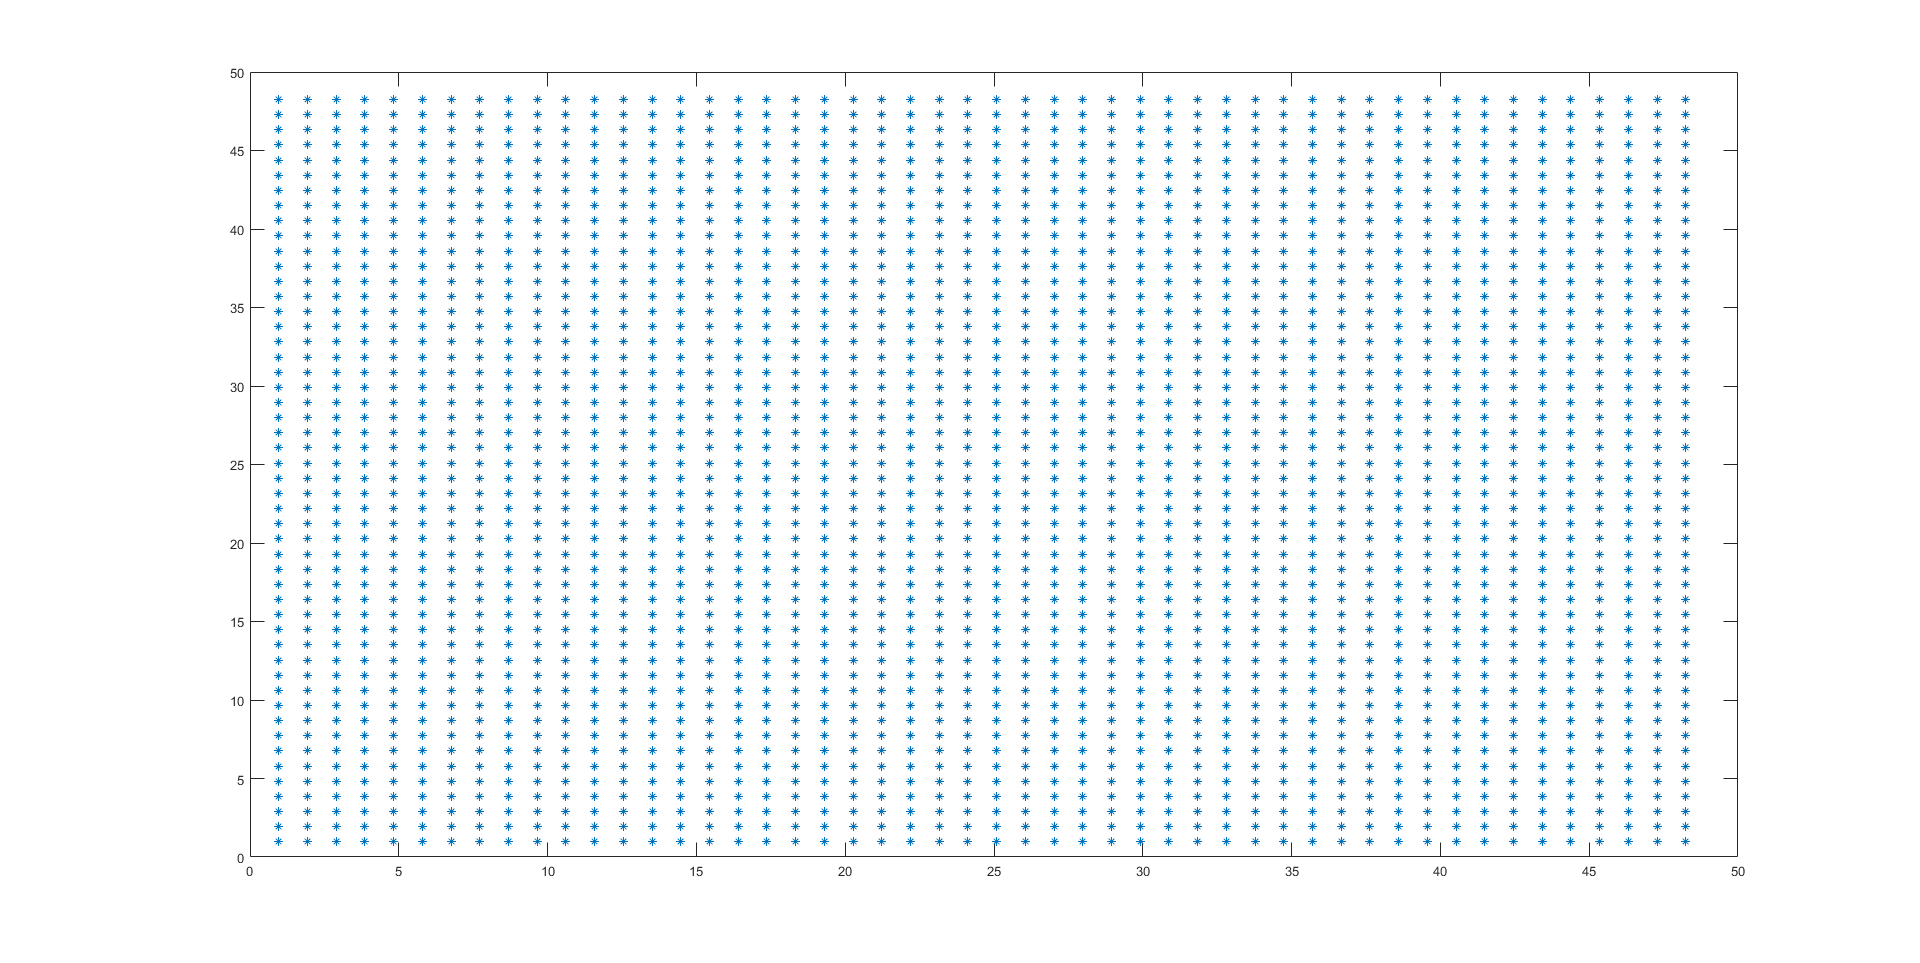
\includegraphics[scale=0.3]{F:/Uni/DatF/datfeksamen/Morten/foerskaelv.png}
\caption{Plot af klods positioner før pertubation}
\end{figure}

\newpage
Hernæst skal vi se hvad der er sket med klodsernes positioner, efter det øverste lag er blevet forskubbet

\begin{figure}[!h]
\centering
\includegraphics[scale=0.3]{F:/Uni/DatF/datfeksamen/Morten/efterskaelv.png}
\caption{Plot af klods positioner efter pertubation}
\end{figure}

hvor følgende information blev outputtet til konsolen for skælvet illustreret ovenfor.\\

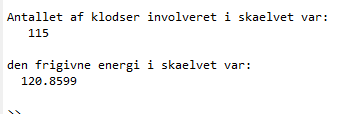
\includegraphics[scale=1]{F:/Uni/DatF/datfeksamen/Morten/consoloutput.png}

Vi har altså både numerisk og visuel represæntation af skælvets størrelse.


\section{Afsluttende}
Modellen viser glimrende, hvordan objekter der er forbundet via fjedre i en struktur, reagerer når én eller flere af disse elementer bliver forstyret af en udefrakommende kræft. Programmet simulerer ganske godt den ønskede model, dog med visse begrænsinger, så som begrænsingen af hvor stor forskydingen af det øvre lag må være før programmet ikke længere giver et brugbart output. Der bliver også givet en idé af hvor meget energi der bliver afsat af skælvet, hvilket er brugbart til, at få fornemmelse af hvor stort skælvet var, fra andre steder end et plot. På trods af at værdien ikke har nogen meningsfuld enhed som det er lige nu.


\end{document}